\subsection{Implémentation d'un système de commande}
Passons maintenant à la descriptions des différentes classes et interfaces du système de commande.

\newcommand{\classname}[1]{\textbf{\texttt{#1}}}
\subsubsection{Structure}
\begin{figure}
 \centering
 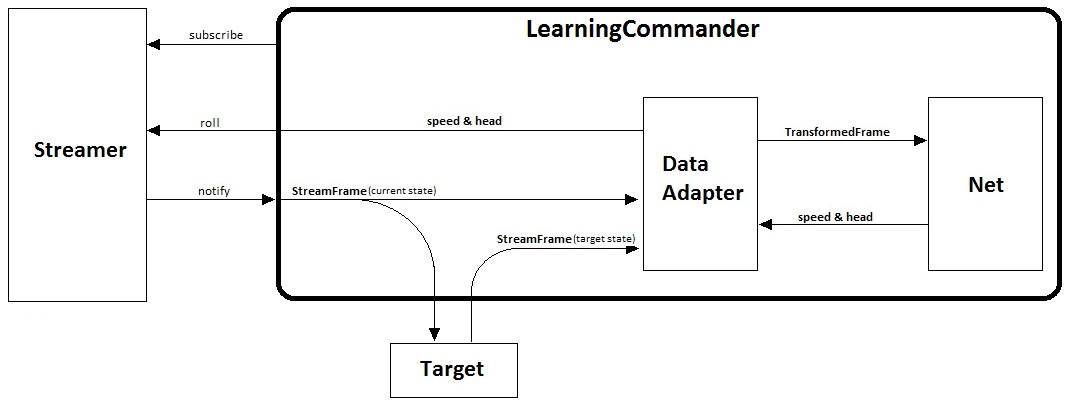
\includegraphics[width=0.8\textwidth]{../figures/commander.jpg}
 \caption{Structure du système de commande}
 \label{fig:commander}
\end{figure}
\begin{figure}
 \centering
 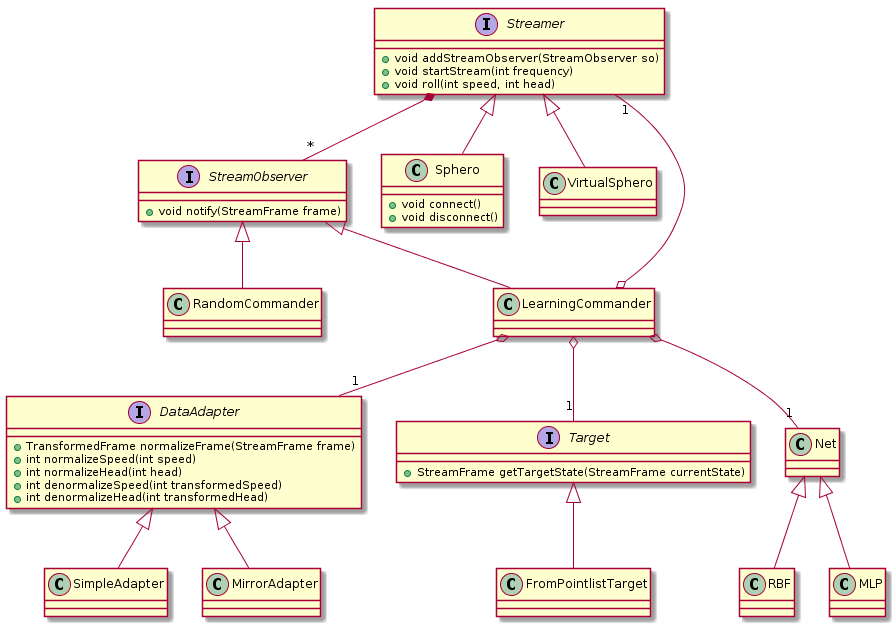
\includegraphics[width=\textwidth]{../../uml/commanderdiag.png}
 \caption{Diagramme de classe dy système de commande.\footnotesize Généré par \href{http://plantuml.com/class-diagram}{plantUML}}
 \label{fig:commanderdiag}
\end{figure}

En résumé, on inscrit le commander par machine learning à un Streamer.
Ensuite on démare le streaming en donnant la fréquence $f$ au Streamer.
Le Streamer va périodiquement notifier le commander d'une nouvelle frame de données issues du streaming.
Le commander va demander au Target l'état cible à atteindre dans $\frac{1}{f}$ secondes d'après l'état actuel du Streamer.
Le commander Passe ensuite l'état actuel et l'état à atteindre dans un DataAdapter qui a pour but de résumer les données et les fournir comme input au réseau de neurones.
Ce DataAdapter se charge aussi de réduire le domaine d'entrée pour avoir une convergence plus rapide.
Le commander récupère le output du réseau de neurones et le passe au DataAdapter qui éffectuera une transformation afin d'obtenir les commandes à envoyer directement au Streamer.
Cette procédure est illustré dans la Figure \ref{fig:commander} est reprend les éléments suivants:
\begin{itemize}
 \item \classname{StreamFrame}: Une structure contenant les données brutes du streaming.
  C'est à dire l'orientation de la Sphero, sa position, son vecteur vitesse et son vecteur d'accélération mais aussi le temps entre la récéption de cette frame et la précédente.
 \item \classname{StreamObserver}: Un objet qui pourra être notifié par un Streamer chaque fois que une \texttt{StreamFrame} est reçue.
  LearningCommander mais aussi le commander par commandes aléatoires sont des StreamObservers. (Figure \ref{fig:commanderdiag})
 \item \classname{Streamer}: Un objet capable de fournir des données issues d'un streaming et les envoyer au StreamObserver qui lui est abonné.
  La Sphero et VirtualSphero sont des streamers. (Figure \ref{fig:commanderdiag})
 \item \classname{Target}: Fourni un état à atteindre d'après l'état actuelle de la Sphero.
 \item \classname{LearningCommander}: Il essaie d'atteindre l'état demandé par Target
 \item \classname{DataAdapter}: Transforme les données de streaming et de l'état à atteindre afin de réduire le domaine d'entrée des données à fournir au réseau de neurones.
  Permet la transformation inverse.
 \item \classname{TransformedFrame}: Une structure contenant les données de streaming mais relatif à la position actuelle de la Sphero et relatif à son orientation,
  avec les données nécessaires sur l'état à atteindre.
 \item \classname{Net}: Le réseau de neurones.
\end{itemize}

\subsubsection{Génération de commande aléatoire}
Afin d'obtenir une base de données qui permetra d'entrainer préalablement le réseau de neurones,
On va d'abord la piloter de manière aléatoire et récuperer ses données de streaming ainsi que les commandes fournies pour y arriver.
Le comportement de ce générateur a un impact important sur la qualitée des données.
Ceci a été observé expérimentalement.

\ssstitle{Éviter les colisions}
Tous les générateurs de commandes aléatoire implémentés durant ce projet ont été conçu pour éviter que la Sphero sorte d'une zone rectangulaire afin d'éviter les colisions.
Lorsque la Sphero dépasse sa zone, des commandes sont envoyées afin que la Sphero fasse demi-tour avec une orientation sufisament proche de celle qui le permetra de revenir dans la zone.
Par exemple, si la Sphero dépasse le bord droit de la zone,
alors l'orientation commandée est dans l'intervale $270 \pm \Delta\text{max}_{\text{about-turn}}$ où $\Delta\text{max}_{\text{about-turn}}$ est un paramètre inférieur à 90 degrés.

\ssstitle{Les erreurs influençant la qualité des données}
Tout d'abord il faut éviter que la différence entre l'orientation actuelle de la Sphero et celle qui est commandée soit supérieur à ce que la Sphero est capable de faire avec sa vitesse angulaire maximale.
En effet, supposons que la Sphero soit capable de changer son orientation de maximum 30 degrés sur un temps de $\frac{1}{f}$ où $f$ est la fréquence de streaming.
Alors toutes les commandes dont le changement d'orientation est entre 30 et 180 degrés, à partir d'un même état initial, aboutiront au même état-cible.
C'est à dire que plusieurs commandes de valeur significativement différentes sont optimales pour atteindre cet état-cible.
Ce qui est mauvais pour la convergence du réseau de neurones.
Pour rappel, si plusieurs outputs sont optimales pour le même input, alors la solution du réseau de neurones ne convergera pas vers un de ces outputs mais vers un outputs de valeur entre ces deux outputs optimals.
Et non seulement cela empêche une bonne convergence mais cela élargi aussi le domaine d'entrée.
Expérimentalement, sans limiter la différence d'orientation, ni le réseau de neurones implémenté, ni le \mlp de Weka, ni celui du package nnet de R ne sont capables de fournir une solution correcte.
Leur comportement est de retourner la moyenne des outputs, quelque soit l'input.\\


Ensuite, afin d'effectuer des trajectoires aléatoires mais naturelles et utiles pour l'apprentissage, il faut pouvoir simuler un humain qui effectuerait des mouvements aléatoires sur une télécommande.
En effet, si la différence d'orientation entre l'état actuelle et l'orientation commandée est purement aléatoire, alors elle alterne rapidement entre positif et négatif.
Ce qui provoque des tremblements, des mouvements balanciers et des trajectoires trop souvent en ligne droite.
Les données de streaming issues d'un tel comportement ne permettaient pas non plus au réseau implémenté au au \mlp de Weka de converger vers une autre solution que la moyenne de tous les outputs.
Pour pouvoir simuler cette commande naturelle, la générateur va d'abord choisir une orientation aléatoire.
Ensuite un nombre d'étape aléatoire.
Soit $N$ le nombre d'étape, soit $d$ la différence d'angle (celle inférieur à 180) entre l'orientation actuelle de la Sphero et la ciblée.
Le générateur va commander une rotation de $\frac{d}{N}$ pour les $N$ prochaines commandes sauf au moment où la Sphero quitte sa zone délimitée.
Le nombre $N$ est généré de sorte à éviter le premier problème cité.
Ensuite, lorsque la Sphero atteind l'orientation cible, elle a une chance sur trois de changer d'orientation cible.
Afin d'éffectuer quand-même des mouvements droits.
La génération de commande sur la vitesse se fait de la même manière.

\subsubsection{Récupération de la trajectoire}
Passons ensuite au commander utilisant le réseau de neurones.
La Sphero ne sera pratiquemment jamais exactement sur la position cible.
Actuellement, pour résoudre ce problème, l'objet Target cherche parmis les points de sa trajectoire, la plus proche de la position actuelle.
Il renvoie ensuite l'état juste après celui dont la position est le plus proche de la position actuelle de la Sphero.
Mais cette technique présente plusieurs inconvénients:
Elle ne permet pas les trajectoires croisées comme les trajectoires en 8.
De plus, la Sphero pourrait dévier assez fort de sa trajectoire cible.
Dans ce cas, la position de la Sphero risque d'être plus proche d'un autre point de la trajectoire que celui qu'il est sensé atteindre.
%\ssstitle{Méthode}
%\ssstitle{Limitation}
%\ssstitle{Solution à la limitation} TODO
\subsubsection{Éditeur de trajectoire}
\begin{figure}
 \centering
 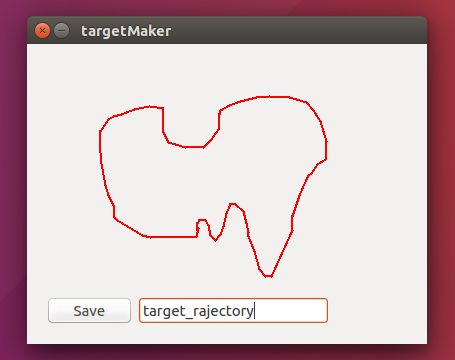
\includegraphics[scale=0.6]{../figures/targettrajectory.png}
 \caption{Éditeur de trajectoire}
 \label{fig:targettrajectory}
\end{figure}
Une interface graphique a été implémentée en Qt afin de créer des trajectoires à la souris. (Figure \ref{fig:targettrajectory})
